% !TEX root = frenetic_programmers_guide.tex

\chapter{Routing}

\section{Design}
\label{routing:design}

Up until now, we've been dealing with OSI Layer 2 technologies -- those that operate at the
Ethernet packet level.  Now we'll step one layer up the stack to Layer 3: Internet Protocol
or IP.  

From the IP perspective, the Internet is just a bunch of LAN's organized into networks, 
then further divided into subnets.  For our purposes, we'll concentrate on
IP Version 4 or IPv4, which is currently the most popular of the two IP versions (the other being
IP Version 6 or IPv6).  

A particular IPv4 address, for example 10.0.1.3, may be part of a subnet
with other hosts.  We may set up a subnet labelled 10.0.1.0/24, which means the first 24 bits
comprise the subnet number, and the last $32 - 24 = 8$ bits are the host number.  In our example, the
subnet number is 10.0.1 and the host is 3.  Because the host number is 8 bits, this means our example
host lives in a subnet with up to 256 neighbors.  Some neighbors are reserved:

\begin{description}
\item[Host 0], in this case 10.0.1.0, usually has no host assigned to it. 
\item[Host 1], in this case 10.0.1.1, is usually the default gateway of the subnet, which we'll see in 
a minute.
\item[Host $n$ - 1], in this case 10.0.1.255, is the subnet broadcast address.
\end{description}

This leaves you with $n$ - 3 ``real'' neighbor hosts.  You can think of a subnet as a gated community
where the most common action is to talk with your neighbors, but not with those outside your
subnet.  To do the latter, you need an intermediary \ldots in IP, that intermediary is a router.

So suppose we have two subnets, each with two hosts, organized like this:

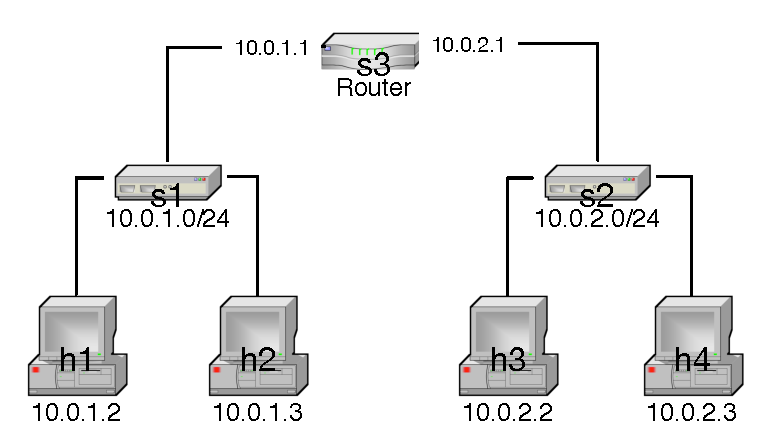
\includegraphics{routing_topo.pdf}

There is no such thing as speaking IP \emph{natively} over a network.  You must speak the wire protocol,
which in most cases is Ethernet.  Because IP applications like your browser and Ping can only speak
in IP addresses, there must be a translation mechanism between IP addresses and Ethernet addresses.
That translation mechanism is Address Resolution Protocol or ARP.  

A typical conversation between two hosts on the same subnet, looks something like this:

\begin{enumerate}
\item Host 10.0.1.2 wants to communicate with 10.0.1.3, but doesn't know it's MAC address.
\item It broadcasts over Ethernet an ARP request, "Who has 10.0.1.3" ?
\item Assuming 10.0.1.3 is up, it sends back an ARP reply, "10.0.1.3 is at 11:22:33:44:55:66", which is
presumably its own MAC address.
\item Host 10.0.1.2 then constructs an Ethernet packet with destination 11:22:33:44:55:66 and sends it off.
\end{enumerate}

We haven't had to think about ARP in previous chapters, because the hosts have seamlessly handled it
for us.  Our L2 learning switch handles Ethernet broadcasts and Ethernet unicasts just fine, so every
part of the conversation above was handled by it seamlessly.

Now, throw a router into the mix and the conversation gets slightly more complicated.  Host IP
stacks now distinguish between hosts on their own subnet and hosts on other subnets.  If
10.0.1.2 wants to talk to 10.0.2.3, the host won't just send out an ARP request for 10.0.2.3 -- it's
on another network.  Hosts can have routing tables to tell it where to direct inter-network
traffic, but in most cases the routing table contains one entry: the default gateway.  The default
gateway is usually set by DHCP, but it's generally a special IP address on the subnet where the
router lives. In this case the conversation becomes:

\begin{enumerate}
\item Host 10.0.1.2 wants to communicate with 10.0.2.3, but doesn't know it's MAC address.  Since
10.0.2.3 is on different subnet, and there's no routing table entry for a subnet including 10.0.2.3,
it decides to send to a default gateway 10.0.1.1
\item It broadcasts over Ethernet an ARP request, ``Who has 10.0.1.1?''
\item The router sends back an ARP reply, "10.0.1.1 is at 11:00:00:00:00:00", which is
the MAC address of the router port hooked into subnet 10.0.1.0/24.
\item Host 10.0.1.1 then constructs an Ethernet packet with destination 11:00:00:00:00:00 and sends it off.
\end{enumerate}

And now the router can do its thing:

\begin{enumerate}
\item The destination IP is 10.0.2.3, and the router knows it has subnet 10.0.2.0/24
on port 2.  But it doesn't know the MAC address of 10.0.2.3.
\item The router broadcasts an ARP request over port 2 ``Who has 10.0.2.3?''
\item That host responds with an ARP reply ``10.0.2.3 is at ff:ee:dd:cc:bb:aa'', which is its 
own MAC address.
\item Router constructs an Ethernet packet with destination ff:ee:dd:cc:bb:aa and sends it off.
\end{enumerate}

A couple of things to notice here:

\begin{itemize}
\item Only IP traffic gets routed.  
\item Only Ethernet sources and destinations are changed in the packet.  The IP addresses stay the same.
\item A router must buffer packets until the ARP replies return.  For subsequent requests, it caches the
IP-to-MAC translation, like a learning switch does with MACs.
\item If the router receives a packet bound for a network not directly connected to it, the router
itself has a default gateway it can send to.  
\end{itemize}

So the router does two basic things: answers ARP requests, and routes
a packet to the ``next hop''.  Of course real routers do much more than that: they maintain routing tables,
translate network protocols, drop blatantly malicious traffic, and so on.  But we'll concentrate 
on the two core router functions here.

\section{Modeling The Topology}
\label{routing:topo}

Every OpenFlow enabled device is called a \emph{switch}, but you should not confuse it
with a traditional L2 switch.  An OpenFlow switch can model just about any network device
including firewalls, load balancers, and -- as we'll see in this chapter -- routers.  

In Chapter \ref{multitswitch_topologies}, we saw two ways of modeling the network topology:
statically with a \netkat{.dot} file and dynamically via Frenetic.  One advantage of a
static topology is you can share it between Mininet and your application.  That 
way you can model more difficult topologies completely, and only change one file
to change the design.  

So here is our DOT file, from \codefilename{routing/topology.dot}:

\inputminted{python}{code/routing/topology.dot}

We've added a few more attributes to accommodate IP.  In particular:

\begin{description}
\item[router] is set to true on the device acting as the router
\item[subnet] desginates the subnet assigned to a particular switch
\item[ip] addresses are assigned to each host 
\end{description}

Here's the GraphViz generated diagram for the above:

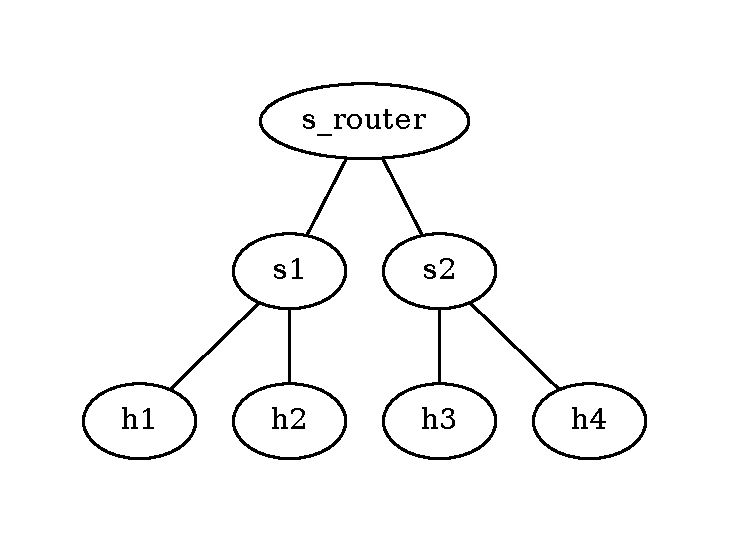
\includegraphics{routing_topology.pdf}

Until now we've been using Mininet's predefined topologies: simple and tree.  We
can define a custom Mininet toplogy by writing some Python code calling the Mininet
API's.  

The following code is in \codefilename{routing/mn_dot_topology.py}:

\inputminted{python}{code/routing/mn_dot_topology.py}

This program relies on the \python{agraph} API, which we used in Chapter \ref{multiswitch}, and 
the Mininet API, documented at: http://mininet.org/api/annotated.html.  The interesting calls are:

\begin{description}
\item[addSwitch()] which adds a new Mininet switch with a particular DPID.
\item[addHost()] which adds a host
\item[addLink()] which adds virtual ``wire'' between a host and a switch, or two switches.
\end{description}

In this program, we're careful to set the port ids to some defaults.  Although that's not
technically necessary, since L2 learning will establish a table of MAC-to-port mappings,
it makes debugging easier.  It's also natural for routers to be configured with subnet-to-port
mappings in advance -- learning this information on the fly is prone to problems.  

To run this Mininet topology, you simply run this python file as root:

\begin{minted}{console}
vagrant@frenetic:~/manual/programmers_guide/code/routing$ sudo python mn_dot_topology.py
*** Removing excess controllers/ofprotocols/ofdatapaths/pings/noxes

  ... a lot of cleanup messages 

*** Cleanup complete.
Unable to contact the remote controller at 127.0.0.1:6633
Network ready
Press Ctrl-d or type exit to quit
mininet>
\end{minted} 

\section{A Better Router}

One of the problems with traditional routing is the ARP process.  The router must have gobs of memory 
to buffer packets waiting for ARP replies \ldots and those replies may never arrive!  But here, SDN 
can help us build a faster, simpler router.

In Chapter \ref{multiswitch_topologies} we saw how a global network view helps us build a loop-free
network without the hassle of spanning tree.  We can use this same global network view to build
routing without relying on ARP.  

The key is in the L2 learning tables.  If 10.0.1.2 wants to communicate with 10.0.2.3, we probably know
both of their MAC addresses.  10.0.1.2 cannot simply address its packet directly to that MAC because
it's not on the same switch (and Ethernet, by itself, is not routable).  But the router can use 
10.0.2.3's MAC address to perform the second hop.  It can skip the buffering and ARP request step
altogether.

But what if the MAC address of 10.0.2.3 is \emph{not} known?  In this case, our smarter router can simply
``outsource'' the problem to the network switch.  It can set the destination MAC address to an 
Ethernet broadcast and send it to switch 2.  Although this temporarily increases network traffic, it's not much
worse than broadcasting an ARP request.  Usually the host responds quickly, causing L2 learning to 
occur.  

Under these conditions, the switches don't need any modification.  When a host needs to send an 
internetwork packet, they always start by sending the packet to the default gateway.  From that 
perspective, the default gateway is no different than any other host.  If the sender knows 
its MAC address, it simply sends it.  If it doesn't, it broadcasts an ARP request for it and the
router responds.  

The router needs to implement two kinds of rules.  The first rule is for learned MACs.  For each
$mac$ and address $ip$, you first determine the router port $rp$.  That can be calculated since
we know which subnet is connected to each router port.  Then we write the rule:

\begin{minted}{python}
Filter(EthTypeEq(0x800) & IP4DstEq(ip)) >> \
  SetEthDst(mac) >> SetPort(rp) 
\end{minted}

Then we write a catch-all rule for any hosts in the subnet that we don't know yet.  Here, $subnet$
and $mask$ are the subnet we're matching and $rp$ is the router port to which it's connected

\begin{minted}{python}
Filter(EthTypeEq(0x800) & IP4DstEq(subnet, mask)) >> \
  SetEthDst("ff:ff:ff:ff:ff:ff") >> SetPort(rp) 
\end{minted}

This appears to overlap with previous rule since a host match like 10.0.1.3 should trigger the 
subnet match of 10.0.1.0/24.  But OpenFlow actually guards against this - if there are multiple 
IP matching rules, the most specific always wins.  So we can \netkat{Union} these
rules together without having to sue \netkat{IfThenElse}.  

Note that unlike switches, no learning occurs in a router.  We rely on the switches to do all the
MAC learning for us, which works well because no hosts directly connect to the router.  However,
we do need to catch all ARP requests so that we can answer requests for the default gateway:

\begin{minted}{python}
Filter(EthTypeEq(0x806) ) >> SendToController("router") 
\end{minted}

Note that we don't need to \emph{answer} all ARP requests, necessarily \ldots and in fact we'll see
ARP requests for intra-network hosts because they are broadcast over the subnet.  We can ignore those
since they'll be answered by the host itself.  The only ones we reply to are those for the default 
gateway.  

\section{Modularization}

When we get done, our network application will perform the job of both the switches and the router.  
Up until now, we have written our applications as one subclass of \python{Frenetic.App}, but here
it makes sense to modularize the application into a switch part and a router part.  We call these
handlers, and they implement the same method signatures that Frenetic applications do.  
They are not subclasses of \python{Frenetic.App} -- making them subclasses would give them each 
their own event loops and asynchronous calls, which simply makes things too complicated.   However, they
could be turned into their own freestanding Frenetic applications simply by making them subclasses.

The main application looks like this, from \codefilename{routing/routing1.py}:

\inputminted{python}{code/routing/routing1.py}

Notice how it creates one NIB, and passes these to both switch and router handlers.  This allows
them to share state.  But learning a new MAC on the switch should trigger a policy recalculation on
the router.  Rather than coding this dependency into the router (which then couples it to the switch 
handler), we handle the recalculation here.  

There's not a lot of code in this app -- most of the actual work is delegated to the handlers
\python{SwitchHandler} and \python{RouterHandler}.  Each handler does two main tasks: (a) review
incoming packets and (b) contribute their portion of the network-wide policy based on the NIB.  
Since the switches and router policies are non-overlapping (they have different \netkat{SwitchEq} filters)
simply \netkat{Union}'ing them together gives you the network-wide policy.  
In this app, all the handler workflow is hard-coded, but you can imagine a more dynamic 
main program that would register handlers and dynamically delegate events based on signatures. 
That's overkill for our routing application.

The NIB looks a lot like the one for multiswitch handling, from \codefilename{routing/network_information_base.py}:

\inputminted{python}{code/routing/network_information_base.py}  

The main addition is a \python{dirty} bit
which learning/unlearning a MAC can set or.  The main handler uses this to determine whether to do 
a wholesale recalculation of the switch and router policies.

The switch handler is virtually identical to the switching application of Chapter \ref{multiswitch}.  
This code is from \codefilename{routing/switch_handler.py}:

\inputminted{python}{code/routing/switch_handler.py}

The main changes are the removal of switch connection code.

The interesting processing happens in \codefilename{routing/router_handler.py}:

\inputminted{python}{code/routing/router_handler.py}

Here you can see the learned MAC policies, the catch-all subnet policies, and the ARP policy are 
installed.  ARP replies are constructed from scratch using the RYU packet library described in
Section \ref{introduction:packet_in}.